
\providecommand{\myrootdir}{..}
\documentclass[\myrootdir/main.tex]{subfiles}

\begin{document}

\chapter{Introduction}
Continuous Integration (CI) has become a common practice in software engineering~\cite{hilton2016usage}.
Many software projects use CI~\cite{hilton2016usage,staahl2014modeling,beller2017oops} to detect bugs early~\cite{vasilescu2015quality,duvall2007continuous}, improve developer productivity~\cite{miller2008hundred,hilton2016usage} and communication~\cite{downs2012ambient}.
A build on a CI server typically compiles and packages the software, executes tests~\cite{beller2017oops} and various kinds of static analyses~\cite{zampetti2017open}.

CI builds produce long and verbose build logs~\cite{beller2017oops}, reporting the progress and results of the steps within the build.
The structure of these logs changes from project to project~\cite{staahl2014modeling} as it depends on the tools and the environment used.
Build logs are a valuable data source for developers and researchers.
Developers read them to analyze why their build failed or how different stages of the build process perform.
Researchers can harvest the information contained in the logs to study the software engineering process of a project~\cite{rausch2017empirical,beller2017oops,seo2014programmers,vassallo2017a-tale}.
However, these two groups can only use the information within the build logs if they can adequately retrieve the information relevant to them.

There are different techniques to retrieve information from CI build logs. Beller et al.\ use regular expressions to analyze the reasons of build failures from Travis CI logs~\cite{beller2017oops}.
Such regular expressions are developed by looking at a few exemplary build logs. Updating them whenever new cases are introduced is a tedious and error-prone task~\cite{michael2019regexes}.
Vassallo et al.\ wrote a custom parser for build logs to gather information for build repair hints~\cite{vassallo2018un-break}.
Recently, Amar et al.\ reduced the number of build log lines for a developer to inspect by creating a diff between the logs from a failed and a successful build~\cite{amar2019mining}.

These approaches have various downsides and strengths:
Regular expressions are exact but difficult to maintain~\cite{michael2019regexes}.
Custom parsers are powerful though fragile towards changes in the log structure.
Taking a diff between failed and successful logs can reduce the information to be processed, but the imprecise output needs to be interpreted by a developer~\cite{amar2019mining}.
At the moment there is only anecdotal evidence on the performance of these techniques and when a technique should be preferred over other alternatives.
Developers and researches currently have little support while choosing which technique to use for a task.

The goal of this thesis is to investigate different chunk retrieval techniques for build logs and describe under which circumstances each techniques is recommended over another.
We aim to characterize different chunk retrieval techniques, as well as the information retrievable from CI build logs.
For \textbf{RQ1}, we analyze which criteria influence the suitability of a chunk retrieval technique for CI build logs.
We implement and evaluate three chunk retrieval techniques:
\begin{itemize}
  \item program synthesis by example using the Microsoft PROSE library (referred to as PBE),
  \item a common text similarity approach (referred to as CTS), and
  \item keyword search (referred to as KWS).
\end{itemize}
\textbf{RQ2} asks under which conditions PBE, CTS and KWS are suited to retrieve information from continuous integration build logs.
\textbf{RQ2} is refined into sub-questions along with the criteria resulting from \textbf{RQ1} and compares their instantiations for the three techniques:
How many training examples a technique needs to perform best (\textbf{RQ2.1}), how structurally diverse the examples can be (\textbf{RQ2.2}) and how accurate the retrieved output is(\textbf{RQ2.3}).
To evaluate PBE, CTS and KWS we create a data set, namely \emph{LogChunks}, which encompasses about 800 log files from 80 repositories.
Each log is labeled with the log part describing the reason a build failed, keywords to search for this log part and a categorization of the labeled log part according to its structural representation within the log.

Our study of the three techniques on \emph{LogChunks} shows that
\begin{itemize}
  \item PBE yields very accurate results when trained with two examples from a single structural category.
  \item CTS shows the best average precision, though precision and recall of a retrieval is hard to determine from the given result.
  A small increase in the number of training examples has no noticeable influence.
  Fewer structural categories improve precision and recall of the retrieval.
  \item KWS has the highest recall of all techniques, however much lower precision.
  It is the technique with the best recall when multiple structural categories are present in the training examples.
\end{itemize}
We recommend PBE for use cases where the desired information is always represented in the same structural way and high confidence in precision and recall of the chunk retrieval is required.
CTS is well suited when the representation of the desired information varies slightly and the output of the chunk retrieval is further processed by a human.
In cases where the textual representation of the desired information in the log is unpredictable or varies greatly, KWS is the best technique to choose.
However, its low precision requires a human to interpret the output of the chunk retrieval.

\paragraph{Our work contributes:}
\begin{itemize}
  %\item A model of the contained and retrievable information in CI build logs.
  %\item A model to characterize chunk retrieval techniques from CI build logs.
  \item A tool unifying several chunk retrieval techniques namely:
        \begin{itemize}
          \item program synthesis from examples using the Microsoft PROSE library (PBE),
          \item a common information retrieval approach using text similarity (CTS), and
          \item a keyword search approach (KWS).
        \end{itemize}
  \item A validated data set of about 800 logs from failed Travis CI builds manually-labelled with:
        \begin{itemize}
          \item the substring of the log describing the reason the build failed,
          \item keywords developers would use to search for these substrings, and
          \item a categorization of the substrings according to their structural representation within the build log.
        \end{itemize}
  %\item A study comparing the effectiveness of the three implemented techniques.
  \item Recommendations for the configuration of each of the investigated chunk retrieval techniques.
  \item Guidelines on choosing a suitable chunk retrieval technique.
\end{itemize}

This thesis first presents an overview of related research, spanning from CI, build log analysis and augmentation to system log processing.
Chapter~\ref{sec:rw} also presents existing work on information extraction and retrieval techniques, as well as program synthesis from examples.
Next, Chapter~\ref{sec:techniques} characterizes chunk retrieval techniques and retrievable information from CI build logs.
It also introduces the three investigated techniques PBE, CTS and KWS\@.
Chapter~\ref{sec:data-set} describes the creation of the \emph{LogChunks} data set collected from failed Travis CI build logs, including the labeling and the validation process.
%Chapter~\ref{sec:implementation} outlines our implementation of the three chosen chunk retrieval techniques and the usage of our unified chunk retrieval tool.
This tool is also used for the comparison described in Chapter~\ref{sec:study}.
Chapter~\ref{sec:discussion} discusses the implications of the study results and recommendations on when PBE, CTS and KWS are most suitable.
Lastly, we conclude and give an overview of further research opportunities in Chapter~\ref{sec:conclusion-fw}.%\\\\

% Following we show selected plots from the study results section. RLR stands for the baseline technique \emph{Random Line Retrieval}:

% \begin{figure}[htbp]
% 		\centering
% 		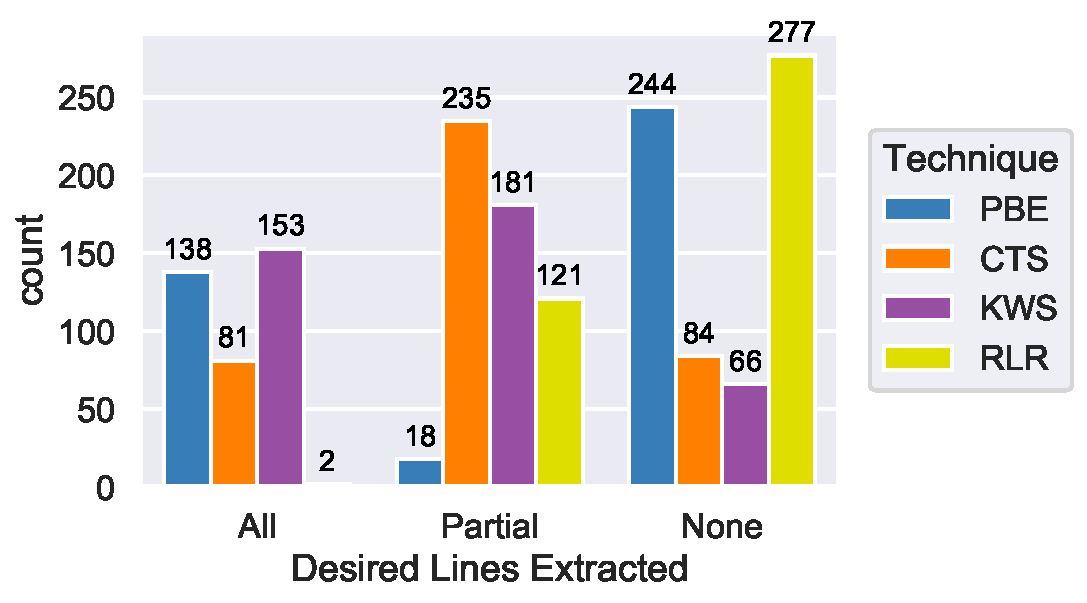
\includegraphics[width=0.75\textwidth, clip]{img/big-study/success-partial-all.pdf}
% 		\caption{Success of chunk retrievals for all techniques}
% 		\label{fig:success-partial-all}
% \end{figure}

% \begin{figure}[htbp]
% 	\centering
% 		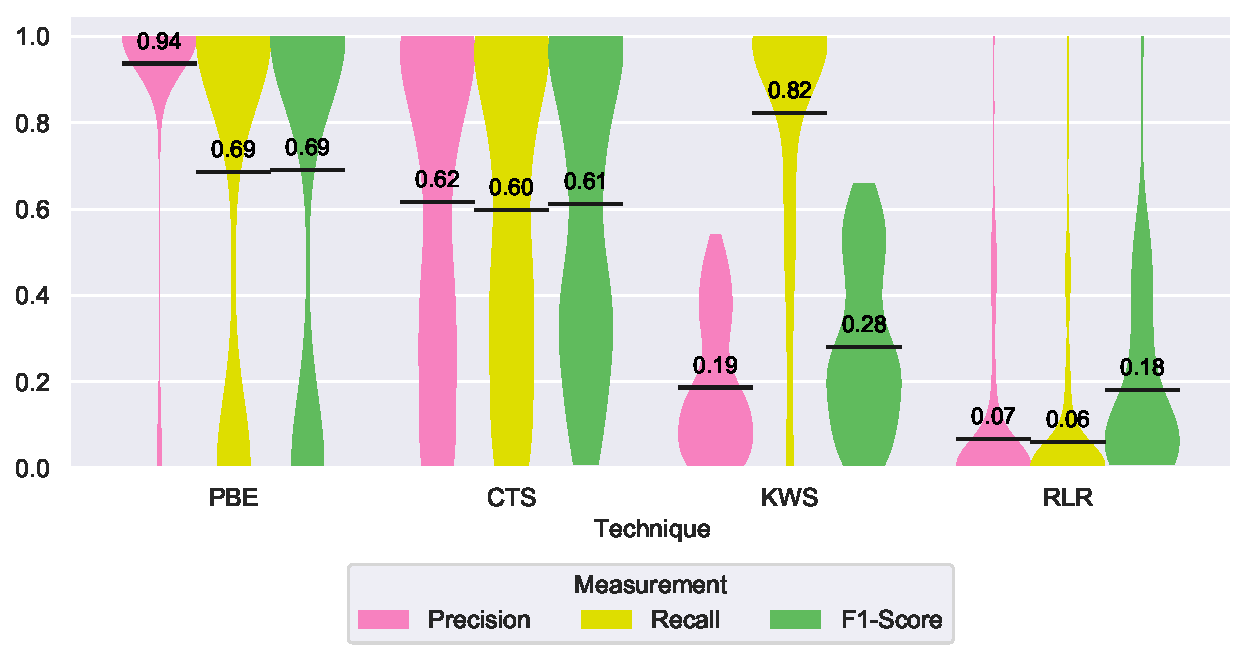
\includegraphics[width=0.75\textwidth, clip]{img/big-study/recall-precision-singlecategory-all.pdf}
% 		\caption{Precision and recall of all techniques compared when training examples are in \emph{one} structural category}
% 		\label{fig:recall-precision-singlecategory-all}
% \end{figure}

% \begin{figure}[htbp]
% 		\centering
% 		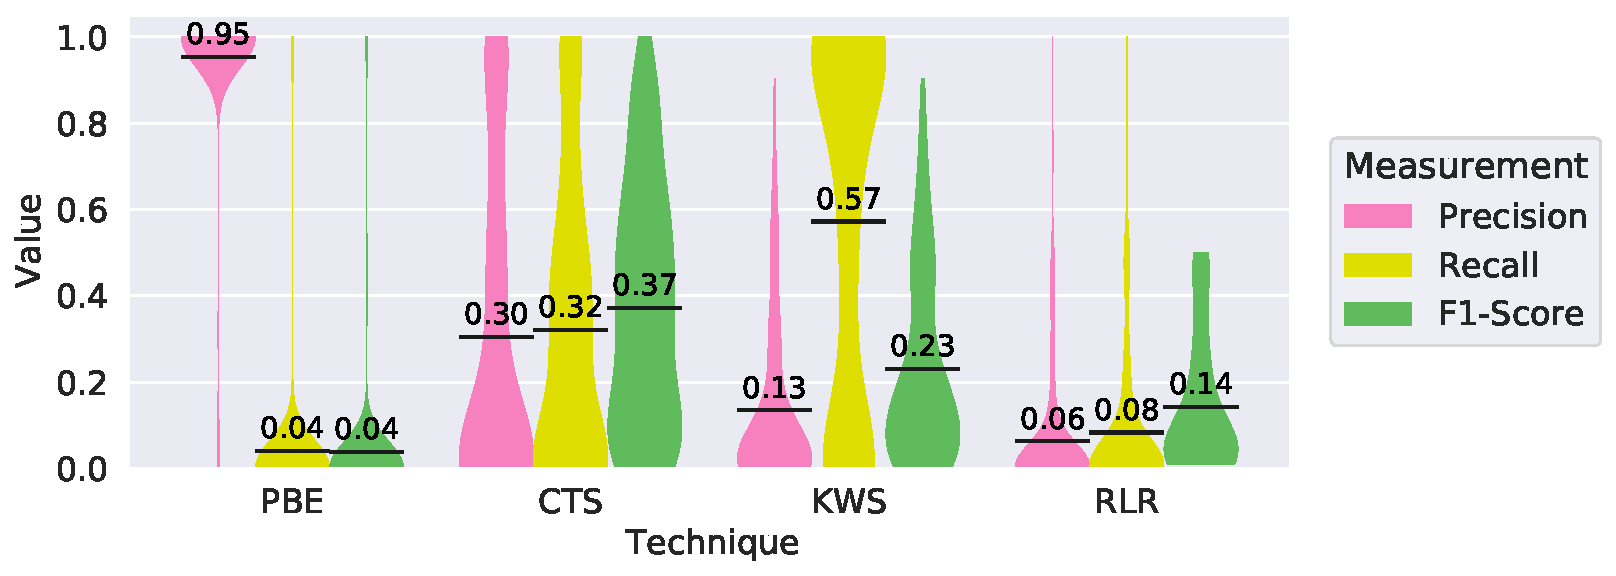
\includegraphics[width=0.75\textwidth, clip]{img/big-study/recall-precision-multicategory-all.pdf}
% 		\caption{Precision and recall of all techniques compared when training examples are in \emph{more than one} structural categories}
% 		\label{fig:recall-precision-multicategory-all}
% \end{figure}

\end{document}


